\setchapterpreamble[u]{\margintoc}
\chapter{Bayesian statistics}
\label{chap:bayesian_statistics}

Let us go back to the problems of statistical inference that we considered in Chapter~\ref{chap:statistical_inference}.
We have data $X$ valued on a measurable space $(E, \cE)$ and a model $\{ P_\theta : \theta \in \Theta\}$ for its distribution, see Definition~\ref{def:statistical_experiment} from Chapter~\ref{chap:statistical_models}.
For the problems of estimation and testing, we can define a set $A$ of \emph{decisions}: for scalar estimation, it is $A = \Theta \subset \R$, while for testing, we have binary decisions, so that $A = \{ 0, 1 \}$.

\section{Elements of decision theory} % (fold)
\label{sec:elements_of_decision_theory}

Given a (measurable) statistical procedure $\delta : E \go A$, we \emph{decide} $\delta(X) \in A$.
In order to assess a decision, we use a \emph{loss function} $\ell : A \times \Theta \go \R$.
This means that if the true parameter is $\theta \in \Theta$ and if we decide $a \in A$, we incur a loss $\ell(a, \theta) \in \R$.

\begin{definition}
	Consider a statistical experiment with data $X \in E$ and a set of parameters $\Theta$, a set $A$ of decisions and a loss function $\ell : A \times \Theta \go \R$. The \emph{risk} of a statistical procedure $\delta : E \go A$ is given by
	\begin{equation*}
		R(\delta, \theta) = \E_\theta[ \ell(\delta(X), \theta)]
	\end{equation*}
	for any $\theta \in \Theta$.
\end{definition}

For the problem of estimation of a scalar parameter, we have $\Theta = \R = A$ and $\ell(\theta', \theta) = (\theta' - \theta)^2$, so that the risk is, in this case, the quadratic risk introduced in Definition~\ref{def:quadratic_risk} from Chapter~\ref{chap:statistical_inference}.
Note that we could consider other losses, such as $\ell(\theta', \theta) = |\theta' - \theta|^p$ for some $p \geq 1$.


Consider now statistical testing with hypotheses $H_0 : \theta \in \Theta_0$ and $H_1 : \theta \in \Theta_1$ where $\{ \Theta_0, \Theta_1 \}$ is a partition of $\Theta$.
Introduce the loss given by
\begin{equation}
	\label{eq:bayes-test-loss}
	\ell(i, \theta) = 0	\quad \text{if} \quad \theta \in \Theta_i \quad \text{ and } \quad \ell(i, \theta) = c_i \quad \text{if} \quad \theta \in \Theta_{1 - i}
\end{equation}
for $i \in \{ 0, 1 \}$ and constants $c_0, c_1 > 0$.
The risk writes in this case
\begin{equation*}
	R(\delta, \theta) =	c_i \P_\theta [\delta(X) = i] \quad \text{when} 
	\quad \theta \in \Theta_{1 - i}
\end{equation*}
for $i \in \{ 0, 1 \}$.
The constants $c_0, c_1 > 0$ allow to tune the importance given to the Type~I and Type~II errors: the approach described here leads to an approach of statistical testing different from the one described in Section~\ref{sec:tests}.


\section{Bayesian risk} % (fold)
\label{sec:bayesian-risk}

Let us go back to the coin flip problem considered in Chapter~\ref{chap:statistical_inference}.
We observe $X_1, \ldots, X_n$ iid distributed as $\ber(\theta)$ for $\theta \in (0, 1)$.
The estimator we introduced back then was the empirical mean $\wh \theta_n = \bar X_n = n^{-1} \sum_{i=1}^n X_i$, and we know from~\eqref{eq:bernoulli-quadratic-risk} that the quadratic risk is given by $R(\wh \theta_n, \theta) = \theta (1 - \theta) / n$ for any $\theta \in (0, 1)$.
But what about the estimator $\wt \theta_n = 0$ ? It is a rather stupid estimator, but if $\theta$ is close to~$0$, it turns out to be a good estimator, and actually, it is easy to see that
$R(\wt \theta_n, \theta) < R(\wh \theta_n, \theta)$ whenever $\theta < 1 / (n + 1)$.
This proves that $\wt \theta_n = 0$ is better than $\wh \theta_n$, when assessed by the quadratic risk, for $\theta$ small enough.%
\sidenote{A longer story hides beneath this simple example: the Stein effect and the Stein estimator, which provably improves the sample average estimator using thresholding, see~\cite{stein1956inadmissibility,lehmann2006theory} for more details on this.}
This very simple example illustrates the fact that it is not possible to find an estimator with an optimal risk for all $\theta \in \Theta$.

%\todo{Exerice on Stein effect ?}

As illustrated above, given two statistical procedures $\delta, \delta'$ for the same problem of statistical inference, we do not have in general that $R(\delta, \theta) < R(\delta', \theta)$ uniformly for $\theta \in \Theta$.
What we can do instead is to consider an \emph{averaged risk}: choose a distribution $\mu$ on $\Theta$ and use it to integrate the risk over $\Theta$.
This distribution is called the \emph{prior distribution} or simply the \emph{prior}.
\begin{definition}[Bayesian risk]
	The Bayesian risk of a procedure $\delta$ associated to the \emph{prior} $\mu$ is given by
	\begin{equation*}
		R_B(\delta, \mu) = \int_{\Theta} R(\delta, \theta) \mu(d \theta) 
		= \int_{\Theta} \mu(d \theta) \int_E \ell(\delta(x), \theta) P_\theta(dx).
	\end{equation*}
\end{definition}
Note that $R_B(\delta, \mu) \leq \sup_{\theta \in \Theta} R(\delta, \theta)$ which means that the Bayes risk is always smaller than the worst-case risk over $\Theta$.
We understand this risk as an average of the risk over $\Theta$ ``weighted'' by the prior distribution $\mu$.
Given a prior $\mu$, the Bayesian risk is a scalar value: we can compare procedures using it and even try to find a procedure that minimizes it.%
\sidenote{We will do it in Section~\ref{sec:posterior_distribution_and_bayes_estimator}, such an estimator is called a Bayesian estimator.}

\begin{example}
	For statistical testing with the loss given by~\eqref{eq:bayes-test-loss}, the Bayesian risk associated to a prior $\mu$ writes
	\begin{align*}
		R_B(\delta, \mu) = \sum_{i \in \{ 0, 1 \}} c_i \int_{\Theta_{1 - i}} \P_\theta[\delta(X) = i] \mu(d \theta),
	\end{align*}
	which is a weighted combination of the Type~I and Type~II errors averaged by the prior $\mu$.
\end{example}

Another interpretation of the Bayesian risk is of utmost importance in Bayesian statistics.
Indeed, we could say that the parameter $\theta$ is \emph{itself a random variable} distributed as $\mu$, that we denote $T$ instead of $\theta$, and that $P_\theta$ is actually the distribution of $X$ ``conditionally'' on $T = \theta$.%
\sidenote[][*-3]{Of course the event $T = \theta$ has zero probability if $T$ is continuous with respect to the Lebesgue measure. We will explain clearly what such a \emph{conditional density} is in Section~\ref{sec:about_conditional_distributions_and_densities} below.}

Assuming that the joint distribution $P_{T, X}$ of $(T, X)$ is given by
\begin{align*}
	P_{T, X}[B \times C] = \P[ T \in B, X \in C] = \int_B \mu(d \theta) \int_C P_\theta(dx),
\end{align*}
we could write the Bayesian risk as an expectation with respect to $P_{T, X}$, since
\begin{equation*}
	R_B(\mu, \delta) = \int_{\Theta} \mu(d \theta) \int_E \ell(\delta(x), \theta) P_\theta(dx) = \E[ \ell(\delta(X), T)].
\end{equation*}
What we need to do now, in order to formalize this, is to explain what a conditional density is, and to explain some useful formulas, such as the Bayes formula for conditional densities.

\section{Conditional densities and the Bayes formula} % (fold)
\label{sec:about_conditional_distributions_and_densities}

Let $X$ and $Y$ be random variables on the same probability space and valued in measurable sets $\cX$ and $\cY$.
Let $\phi$ be a measurable function such that $\phi(X)$ is integrable. 
Let us recall that we can define the conditional expectation $\E [\phi(X) | Y]$ as the random variable $r(Y)$ (for some measurable function $r$, almost surely unique) such that
\marginnote{We assume here that the reader is familiar with the definition of the conditional expectation.}
\begin{equation}
	\E[\phi(X) \varphi(Y)] = \E[ r(Y) \varphi(Y)]
\end{equation}
for any measurable and bounded function $\varphi$.
The particular value $r(y)$ for some $y \in \cY$ is denoted $\E[\phi(X) | Y = y]$. 
We know that
\begin{align*}
	\E[\phi(X) h(Y) | Y] &= h(Y) \E[ \phi(X) | Y]
\end{align*}
almost surely, for any measurable function $h$ such that $h(Y)$ and $\phi(X) h(Y)$ are integrable, and we have also
\begin{align}
	\E [\E[ \phi(X) | Y]] = \E[\phi(X)].
\end{align}
Finally, we have $\E[\phi(X) | Y] = \E[\phi(X)]$ whenever $X$ and $Y$ are independent.
Let us suppose now that the joint distribution $P_{X, Y}$ of $(X, Y)$ has a density $p(x, y)$ with respect to a product of dominating measures $\nu_X \otimes \nu_Y$ on $\cX \times \cY$.
We can define the marginal densities of $X$ and $Y$ as
\begin{equation}
	\label{eq:bayes-marginal-densities}
	p_X(x) = \int_{\cY} p(x, y) \nu_Y(d y) \quad \text{and} \quad
	p_Y(y) = \int_{\cX} p(x, y) \nu_X(d x),
\end{equation}
so that we have
\begin{align*}
	\E[\phi(X)] &= \int_{\cX} \phi(x) P_X(dx) = \int_{\cX} \phi(x) p_X(x) \nu_X(dx) \\ 
	\E[\varphi(Y)] &= \int_{\cY} \varphi(y) P_Y(dy) = \int_{\cY} \varphi(y) p_Y(x) \nu_Y(dy)
\end{align*}
for any $\phi$ and $\varphi$ such that $\phi(X)$ and $\varphi(Y)$ are integrable. 
Let us introduce 
\begin{equation*}
	\cY_0 = \big\{ y \in \cY : p_Y(y) = 0 \big\}
\end{equation*}
and remark that
\begin{align*}
	P_{X, Y} [ \cX \times \cY_0 ] 
	&= \int_{\cX \times \cY_0} p(x, y) \nu_X(dx) \nu_Y(dy) \\
	&= \int_{\cY_0} \nu_Y(dy) \int_{\cX} p(x, y) \nu_X (dx) \\
	&= \int_{\cY_0} p_Y(y) \nu_Y(dy) = 0.
	\marginnote{Using~\eqref{eq:bayes-marginal-densities}}
\end{align*}
Given any probability density $q$ on $\cX$ with respect to $\nu_X$, we can define
\begin{equation}
	\label{eq:cond-density-definition}
	p_{X | Y}(x | y) := \frac{p(x, y)}{p_Y(y)} \ind{\cY_0^\complement}(y) + q(x) \ind{\cY_0}(y),
\end{equation}
so that all the versions of $p_{X | Y}$ associated to the choice of $q$ are equal $P_{X, Y}$-almost surely.
Moreover, we can check immediately that $\int_{\cX} p_{X | Y}(x | y) \nu_X(dx) = 1$, so that it is a probability density with respect to $\nu_X$ on $\cX$.
Now, if we define
\begin{equation*}
	r'(y) = \int_{\cX} \phi(x) p_{X | Y}(x | y) \nu_X(dx),
\end{equation*}
we can write, for any measurable and bounded $\varphi$, that
\begin{align*}
	\E[ &r'(Y) \varphi(Y)] \\
	&= \int_{\cY} r'(y) \varphi(y) p_Y(y) \nu_Y(dy) \\
	\marginnote{Using the definition of $r'$, Fubini and~\eqref{eq:cond-density-definition}}
	&= \int_{\cY_0^\complement} \varphi(y) p_Y(y) \nu_Y(dy) 
	\int_{\cX} \phi(x) \frac{p(x, y)}{p_Y(y)} \nu_X(dx) \\
	\marginnote{Using the fact that $P_{X, Y}[\cX \times \cY_0] = 0$}
	&= \int_{\cX \times \cY} \phi(x) \varphi(y) p(x, y) \nu_X(dx) \nu_Y(dy) \\
	&= \E[ \phi(X) \varphi(Y)].
\end{align*}
This corresponds to the definition of the conditional expectation, which is almost surely unique, so that we proved that $r = r'$ almost surely.
Now, we know that we can compute a conditional expectation using the formula
\begin{equation*}
	\E[\phi(X) | Y = y] = r(y) = \int_{\cX} \phi(x) p_{X | Y}(x | y) \nu_X(dx).
\end{equation*}
The density $p_{X | Y}$ is called the \emph{conditional density} of $X$ \emph{knowing} $Y$.

% We can define in the exact same way $p_{Y | X}$ and $\P_{X | Y}$ uniquely on the set $\{ y : p_Y(y) > 0 \}$.
% As explained above the complement $\{ y : p_Y(y) > 0 \}^\complement$ has mass equal to $0$: this has no iincidence since conditional expectation are themslef uniquely defined up to a negligable set .

% We call $\P_{X | Y}$ the conditional distribution of $X$ conditionally on $Y$ and $p_{X | Y}(x | y)$ the density of $X$ ``conditionally on $Y=y$''. 
We can define in the exact same way $p_{Y | X}$, the conditional density of $Y$ knowing $X$, and by construction of $p_{X | Y}$ and $p_{Y | X}$, we have that the following equalities
\begin{equation}
	\label{eq:cond-density-formula}
	p(x, y) = p_{X | Y}(x | y) p_Y(y) = p_{Y | X}(y | x) p_X(x)
\end{equation}
hold $P_{X, Y}$-almost surely.
From these equalities we can deduce that
\begin{equation*}
	p_{X | Y}(x | y) = \frac{p(x, y)}{p_Y(y)} = \frac{p_{Y | X}(y | x) p_X(x)}{\int_{\cX} p(x', y) \nu_X(dx')}
	\marginnote{recalling that $P_{X, Y}[\cX \times \cY_0] = 0$}
\end{equation*}
holds $P_{X, Y}$-almost surely, which leads, using again~\eqref{eq:cond-density-formula}, to the Bayes formula
\begin{equation}
	\label{eq:bayes-formula-conditional-densities}
	p_{X | Y}(x | y) = \frac{p_{Y | X}(y | x) p_X(x)}{\int_{\cX} p_{Y | X}(y | x') p_X(x') \nu_X(dx')},
\end{equation}
that holds, once again, $P_{X, Y}$-almost surely.
This is a remarkable formula, since it allows to \emph{reverse the conditioning}: we can write the conditional density of $X$ knowing $Y$ as a function of the conditional density of $Y$ knowing $X$.
This formula is at the core of Bayesian statistics, as explained in the next Section.


\section{Posterior distribution and Bayes estimator} % (fold)
\label{sec:posterior_distribution_and_bayes_estimator}

Let us go back to the setting introduced in Section~\ref{sec:bayesian-risk}.
We have data $X$ and a statistical model $\{ P_\theta : \theta \in \Theta \}$.
We consider a prior distribution $\mu$ on $\Theta$.
We assume that $\mu$ has a density $p(\cdot)$ with respect to a measure $\lambda$ on $\Theta$, namely $\mu(d \theta) = p(\theta) \lambda(d \theta)$ and that $P_\theta$ has a density that we will denote as $p(\cdot | \theta)$ with respect to a measure $\nu$ on $E$.
\marginnote[*-3]{Using the same letter for both the density of $\mu$ (namely $\theta \mapsto p(\theta)$) and the density of $P_\theta$ (namely $x \mapsto p(x | \theta$)) might look like a bad idea, but it will lead to very nice notations in what follows, and it won't lead to any ambiguity.}
We want to apply Bayesian reasoning: the density $p(\cdot | \theta)$ of the data is understood as a  conditional density of $X$ ``knowing the parameter $\theta$''.


\paragraph{The posterior distribution.} % (fold)

% paragraph paragraph_name (end)

In order to formalize this, we introduce a random variable $T$ distributed as $\mu$, and
we apply~\eqref{eq:cond-density-formula} in order to express the joint density of $(X, T)$ through the product of the conditional density of $X | T$ and the density of $T$:
\begin{equation}
	\label{eq:joint-as-conditional-distribution}
	\marginnote{Which holds $P_{X, T}$-almost surely.}
	p_{X, T}(x, \theta) = p_{X | T}(x | \theta) p_T(\theta) = p(x | \theta) p(\theta).
\end{equation}
We can only proceed like this to express $p_{X, T}$, since what we are given is the prior density $p(\cdot)$ and the model, namely the density $p(\cdot | \theta)$.
We know that the marginal density of $X$ can be computed as
\begin{equation*}
	p_X(x) = \int_\Theta p_{X, T}(x, \theta) \lambda(d \theta) 
	= \int_\Theta p(x | \theta) p(\theta) \lambda(d \theta).
\end{equation*}
Now, using the Bayes formula~\eqref{eq:bayes-formula-conditional-densities}, we can \emph{reverse the conditioning}, and define what we call the \emph{posterior density}
\begin{equation*}
	p(\theta | x) := p_{T | X}(\theta | x) = \frac{p_{X, T}(x, \theta)}{p_X(x)} 
	=  \frac{p(x | \theta) p(\theta)}{\int_\Theta p(x | \theta') p(\theta') \lambda(d \theta')}.
\end{equation*}
This formula expresses the conditional density of the parameter $\theta$ knowing the data $x$ (more formally the conditional density of $T$ knowing $X$) through the model (the conditional density of $X$ knowing $T$) and the prior (the density of $T$) that are both known and chosen beforehand.
Let us wrap-up what we constructed in the following definition.

% We saw in ??? that the joint distribution $Q$ of $(T, X)$ is defined through its marginal distribution $g$ of $T$ and the conditional density $f(x | \theta)$ of $X$ conditionally on $T = \theta$ (hence the notation $f(x | \theta)$), so that
% \begin{equation*}
% 	Q(d \theta, dx) = g(\theta) f(x | \theta) (\lambda \otimes \nu) (d\theta, dx). 	
% \end{equation*} 
% The marginal density $\bar f$ of $X$ can be obtained by integrating with respect to $\theta$:
% \begin{equation*}
% 	\bar f(x) = \int_{\Theta} f(x | \theta) g(\theta) \lambda(d \theta)
% \end{equation*}
% and the conditional density of $T | X = x$ can therefore we written as
% \begin{equation*}
% 	g(\theta | x) = \frac{f(x | \theta) g(\theta)}{\bar f(x)} = \frac{f(x | \theta) g(\theta)}{\int_{\Theta} f(x | \theta') g(\theta') \lambda(d \theta')}.
% \end{equation*}
% If is the density of the conditional distribution denoted $Q_x$ of $T | X = x$.
% We simply used here the \emph{Bayes formula} on conditional densities in order to reverse the order of the conditionning: we expressed $T | X$ from $X | T$ since the distribution of $X | T$ is specified by the model we considered

\begin{definition}
	\label{def:posterior-distribution}
	Consider a \emph{prior} $\mu(d \theta) = p(\theta) \lambda(d \theta)$ and a model $P_\theta(dx) = p(x | \theta) \nu(dx)$ for $\theta \in \Theta$, and the corresponding joint distribution $P(dx, d\theta) = p(x | \theta) p(\theta) \nu(dx) \lambda(d \theta)$.
	The \emph{posterior distribution} is the distribution with density
	\begin{equation*}
		p(\theta | x) = \frac{p(x | \theta) p(\theta)}{\int_\Theta p(x | \theta') p(\theta') \lambda(d \theta')}
	\end{equation*}
	with respect to $\lambda$. 
	It is well-defined and unique for $P$--almost all $(x, \theta)$.
\end{definition}

The Bayesian reasoning is therefore as follows: choose a prior density $p(\theta)$ and a model $p(x | \theta)$ for the data $x$ knowing the parameter $\theta$.
Then, compute%
\sidenote{or approximate it using numerical methods, whenever the posterior distribution cannot be  computed explicitly}%
the posterior distribution $p(\theta | x)$ of $\theta$ knowing the data $x$. 
A nice aspect of this approach is that we can quantify uncertainty right out of the box, since instead of an estimator $\wh \theta_n$ (which is, given data, a single value), we obtain a full posterior distribution $p(\theta | x)$, which takes into account the data $x$ that we observed.
However, such a reasoning is of course only possible when we know how to choose a prior, and when we are able to compute exactly or to approximate efficiently the posterior.
\sidenote{This is the main criticism with Bayesian methods: beyond simple models and conjugate distributions (more on this later), the computation of the posterior is not explicit and requires approximation algorithms that can be numerically expensive, or can depart significantly from the original model, see for instance Chapters~9 and~10 in~\cite{bishop2006pattern}.}

\paragraph{The Bayes estimator.} % (fold)

% paragraph the_bayes_estimator_ (end)
% We do ``as if'' $\theta$ where random and with distribution $\mu$.
% The distribution $P_\theta$ becomes the conditional distribution of $X | T = \theta$, namely
% \begin{equation*}
% 	P_\theta[A] = \E [\ind{A}(X) | T = \theta],
% \end{equation*}
% or even $P_T[A] = \E [\ind{A}(X) | T]$.

% In what follows, we will assume that we have a dominating measure $\lambda$ on $\Theta$ such that $\mu = g \cdot \lambda$ where $g$ is the density of $T$ on $\Theta$ with resoect tp $\lambda$ (often $\lambda$ is the lEbuesgue measure).
% We suppose also that thre is a measure $\nu$ on $E$ for which $P_\theta = f(\cdot | \theta) \cdot \nu$ where similarly $\frac{d P_\theta}{d \nu} = f(x | \theta)$. 
% We use here the notation $f(\cot | \theta)$ instead of $f_\theta$ to stress that it will correspond to a conditional density.
% We need at this point to classify things about conditional distributions and conditional densities.


Let us consider the estimation problem where $A = \Theta \subset \R$ and use the Bayes risk to assess the error of an estimator $\delta : E \go \Theta$.
Arguably, an optimal Bayesian estimator should minimize the Bayes risk, and a beautiful aspect of the Bayesian approach is that such a minimizer can be defined precisely.
Indeed, we can rewrite the Bayes risk as follows:
\begin{align*}
	\marginnote{using~\eqref{eq:joint-as-conditional-distribution}}%
	R_B(\delta, \mu) &= \int_{\Theta} \int_E \ell(\delta(x), \theta) p(x | \theta) p(\theta) \nu(dx) \lambda(d\theta)  \\
	\marginnote{Using Fubini and since we know that $p(x | \theta) p(\theta) = p(\theta | x) p_X(x)$ almost surely}%
	&= \int_E p_X(x) \nu(dx) \int_{\Theta} \ell(\delta(x), \theta) p(\theta | x) \lambda(dx).
\end{align*}
What is remarkable with this rewriting is that in order to minimize $R_B(\delta, \mu)$, we need to minimize, for any fixed $x \in E$, the quantity
\begin{equation*}
	\marginnote{Once again, $T$ is a random variable with distribution $\mu(d\theta) = p(\theta) \lambda(d\theta)$}
	\int_{\Theta} \ell(\delta(x), \theta) p(\theta | x) \lambda(d \theta) =
	\E [\ell(\delta(X), T) | X = x],
\end{equation*}
namely the expectation of the loss with respect to the posterior distribution given by Definition~\ref{def:posterior-distribution}.
This leads to the following definition of a Bayes estimator.
\begin{definition}
	Given a prior $\mu(d \theta) = p(\theta) \lambda(d \theta)$, a model $P_\theta(dx) = p(x | \theta) \nu(dx)$ and a loss $\ell$, any estimator $\wh \theta(X)$ defined as
	\marginnote{such an estimator is not necessarily unique}
	\begin{equation*}
		\wh \theta(x) \in \argmin_{t \in \Theta} \int_{\Theta} \ell(t, \theta) p(\theta | x) \lambda(d \theta) = \argmin_{t \in \Theta} \E[\ell(t, T) | X = x],
	\end{equation*}
	namely a minimizer of the expectation of the loss with respect to the posterior distribution, is called a \emph{Bayes} or a \emph{Bayesian estimator}.
\end{definition}
For the square loss $\ell(\theta', \theta) = (\theta' - \theta)^2$, the Bayes estimator is given by the expectation of the posterior distribution.
Indeed, it is easy to see that
\begin{equation}
	\label{eq:bayesian-estimator-square-loss}
	\wh \theta(x) = \argmin_{t \in \R} \int_\Theta (t - \theta)^2 p(\theta | x) 
	\lambda(d \theta) = \int_\Theta \theta p(\theta | x) \lambda(d \theta).
\end{equation}
If $\ell(\theta', \theta) = |\theta' - \theta|$, we can see that
\begin{equation*}
	\wh \theta(x) = \argmin_{t \in \R} \int_\Theta |t - \theta| p(\theta | x) \lambda(d \theta) = F_{x}^{-1}(1/2),
\end{equation*}
where $F_{x}^{-1}(1/2)$ is the \emph{median} of the posterior distribution.
Here, the notation $F_x^{-1}$ stands for the generalized inverse of the distribution function $F_x(\theta) = \int_{-\infty}^\theta p(\theta' | x) \lambda(d \theta')$ of the posterior distribution.%
\sidenote{This comes from the fact that if $X$ is an integrable real random variable with distribution function $F$, a minimizer of $t \mapsto \E|X - t|$ is given by the median $F^{-1}(1/2)$ of $X$.}

\begin{recipe}
	On some examples, we can compute explicitly the posterior distribution.
	Given the data density $p(x | \theta)$ and the prior density $p(\theta)$, the joint density of the data and the prior is $p(x | \theta) p(\theta)$ and we know from Definition~\ref{def:posterior-distribution} that the posterior density is proportional to the joint density, namely 
	\begin{equation*}
		p(\theta | x) = \mathrm{constant}(x) p(x | \theta) p(\theta),
	\end{equation*}
	where $\mathrm{constant}(x) =  1 / \int_\Theta p(x | \theta) p(\theta) \lambda(d \theta)$. 
	So, using the fact that the integral of the posterior density with respect to $\theta$ equals~$1$, we can try to identify directly the posterior distribution by having a careful look at $p(x | \theta) p(\theta)$, together with some coffee, and looking for a density with respect to $\theta$.
\end{recipe}

\section{Examples} % (fold)
\label{sec:bayesian-examples}


Let us give some standard examples of priors and data distributions where can apply this recipe.

\subsection{How to choose a restaurant ? (Bayesian coin flip)}
\label{sub:bayesian-coin-flip}


The first example is, once again, a coin flip, but this time with a Bayesian flavor.
Consider the data distribution $X \sim \bin(n, \theta)$, namely the model with density
\begin{equation*}
	p(x | \theta) = \binom{n}{x} \theta^x (1 - \theta)^{n-x} \ind{\{ 0, \ldots, n\}}(x)	
\end{equation*}
with respect to the counting measure $\nu$ on $\N$ and the \emph{flat prior} on $\theta$ with distribution $\uni([0, 1])$ on $\theta$, namely a density
\begin{equation*}
	p(\theta) = \ind{[0, 1]}(\theta)
\end{equation*}
with respect to the Lebesgue measure $\lambda$.

\begin{marginfigure}
	
\includegraphics{restos.png}
	\caption{How to choose a restaurant? Is a restaurant with a good rating but few rates better than a restaurant with a slightly worse rating but more rates?}
	\label{fig:restaurants}
\end{marginfigure}
This model can be useful to help us choose a restaurant: given a restaurant, $\theta$ is the unknown probability that a customer is happy ($1$) or unhappy ($0$) with it and $n$ is the number of customers who gave their (binary) opinion.
We have no prior information on $\theta$, so we consider the flat prior.
For each restaurant, we observe the percentage of happy customers (rescaled to a 0 to 5 stars rating in Figure~\ref{fig:restaurants}) and the number $n$ of customers who rated it, so $X$ stands here for the number of happy customers among the $n$ who rated it. 
Assuming that the customers opinions are independent, we have $X \sim \bin(n, \theta)$.
The question is the following: how can we choose a restaurant? Is a restaurant with a good rating but few rates better than a restaurant with a slightly worse rating but more rates?

Using the previous recipe, we know that the density of the posterior distribution is proportional to the density of the joint distribution of the data and prior
\begin{equation*}{}
	p(x, \theta) = p(x | \theta) p(\theta) = \binom{n}{x} \theta^x (1 - \theta)^{n - x} \ind{[0, 1]}(\theta) \ind{\{ 0, \ldots, n\}}(x)
\end{equation*}
with respect to the product measure $\nu \otimes \lambda$.
This means that the posterior density is proportional to $\mapsto \theta^x (1 - \theta)^{n - x} \ind{[0, 1]}(\theta)$. 
We recognize the density
\begin{equation*}
	\theta \mapsto \frac{1}{\beta(a, b)} \theta^{a-1} (1 - \theta)^{b-1} \ind{[0, 1]}(\theta)
\end{equation*}
 of the $\bet(a, b)$ distribution, that we introduced in Section~\ref{sub:some_classical_distributions} of Chapter~\ref{chap:linear_regression},
where we recall that $\beta(a, b) = \int_0^1 t^{a-1} (1 - t)^{b-1} d t = \Gamma(a) \Gamma(b)  / \Gamma(a + b)$.
Therefore, we know that the posterior distribution is $\bet(x + 1, n - x + 1)$, namely
\begin{equation*}
	p(\theta | x) = \frac{1}{\beta(x + 1, n - x + 1)} \theta^{x} (1 - \theta)^{n-x} \ind{[0, 1]}(\theta)
\end{equation*}
If $B \sim \bet(a, b)$, we know that
\begin{equation*}
	\E[Z] = \frac{a}{a + b} \quad \text{and} \quad \var[Z] = \frac{ab}{(a + b)^2 (a + b + 1)}.
\end{equation*}
If we consider the square loss for the estimation of $\theta$, we know from Equation~\eqref{eq:bayesian-estimator-square-loss} that the Bayesian estimator is given by the expectation of the posterior, namely
\begin{equation*}
	\wh \theta = \frac{X + 1}{X + 1 + n - X + 1} = \frac{X + 1}{n + 2}.
\end{equation*}
Note the difference with the \emph{frequentist} (non-Bayesian) estimator $X / n$ that we considered all along Chapter~\ref{chap:statistical_inference} (it was denoted $S_n / n$ back then).
This estimator gives a cute Bayesian answer to the restaurant selection problem.
This estimator is also known as the Laplace's \emph{rule of succession} (see~\sidecite{rule-of-successino} and Figure~\ref{fig:rule-of-succession}).
\begin{marginfigure}[*2]
	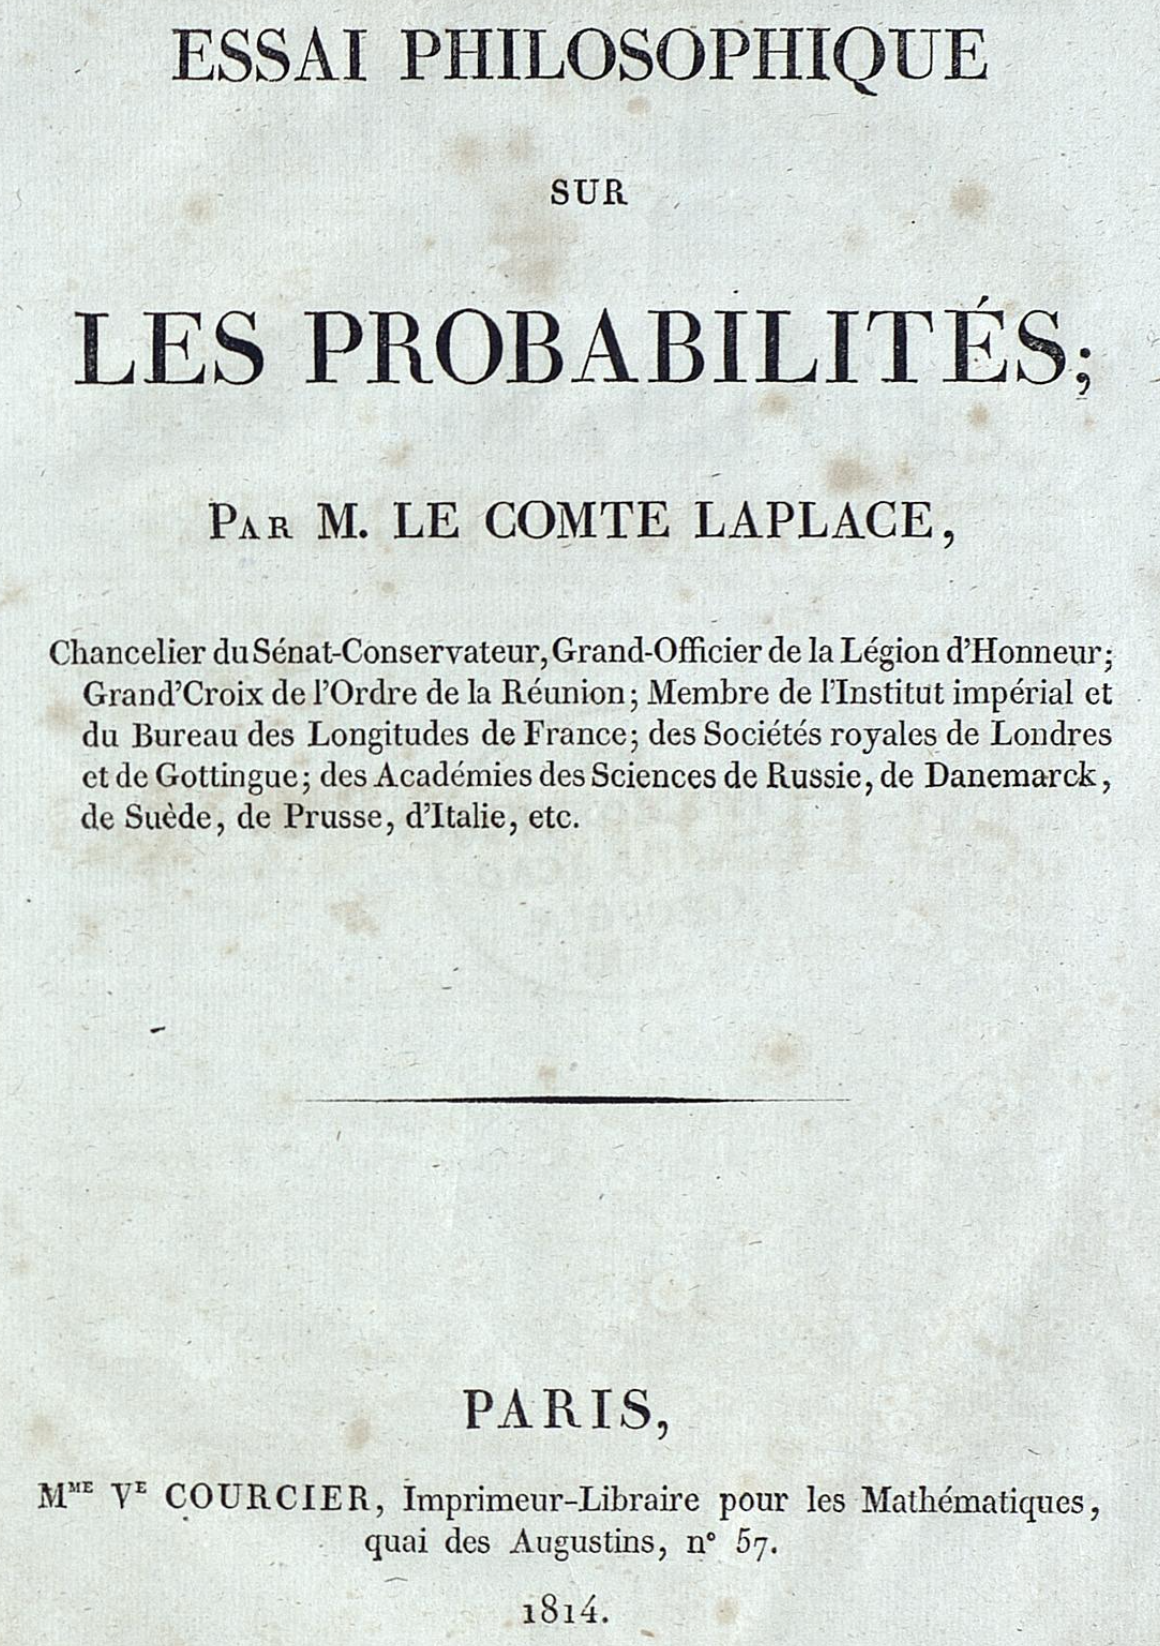
\includegraphics{laplace.png}
	\caption{``Essai philosophique sur les probabilités'' by Pierre-Simon Laplace (1814) in which is introduced the \emph{rule of succession} formula in order to ``solve'' the sunrise problem (What is the probability that the sun will rise tomorrow ?).}
	\label{fig:rule-of-succession}
\end{marginfigure}

Using the bias-variance formula~\eqref{eq:bias-variance-decomposition} from Chapter~\ref{chap:statistical_inference}, we can compute the quadratic risk of $\wh \theta$ as follows:
\begin{align*}
	\E_\theta[ (\wh \theta - \theta)^2] &= \var_\theta[\wh \theta] + (\E_\theta[\wh \theta] - \theta)^2 \\
	&= \frac{n \theta(1 - \theta)}{(n + 2)^2} + \Big(\frac{1 - 2 \theta}{n + 2} \Big)^2 \\
	&= \frac{n \theta - n \theta^2 + 1 - 4 \theta + 4 \theta^2}{(n+2)^2},
\end{align*}
so that the Bayes risk with uniform prior $\mu(d \theta) = p(\theta) d\theta$ where $p(\theta) = \ind{[0, 1]}(\theta)$ is given by
\begin{align*}
	R_B(\wh \theta, \mu) &= \int_0^1 \E_\theta[ (\wh \theta - \theta)^2] d \theta 
	= \frac{1}{6(n+2)}.
\end{align*}
Using the exact same arguments, it is easy to see that if we use the prior distribution $\bet(a, b)$ instead of $\uni([0, 1])$ (which is a particular case, since $\uni([0, 1]) = \bet(1, 1)$) the posterior distribution is given by
\begin{equation*}
	p(\theta | x) = \bet(a + x, b + n - x + b),
\end{equation*}
which leads to a Bayesian estimator (for the square loss) given by
\begin{equation*}
	\wh \theta = \frac{X + a}{n + a + b}.
\end{equation*}
In this example, the prior and the posterior both belong to the family of $\bet$ distributions. 
In such a case, we say that the $\bin$ and $\bet$ distributions are \emph{conjugated}, which corresponds to a situation where the posterior distribution can be \emph{explicitly} computed.
\begin{definition}[Conjugated distributions]
	Given a prior $\mu(d \theta) = p(\theta) \lambda(d \theta)$ and a model $P_\theta(dx) = p(x | \theta) \nu(dx)$, we say that the distributions of the prior and of the model are \emph{conjugated} whenever the prior and the posterior distribution belong to the same family of distributions.
\end{definition}


\subsection{Gaussian sample with a Gaussian prior}

Another classical example is with the Gaussian distribution.
Consider data $X_1, \ldots, X_n$ iid with $\nor(\theta, \sigma^2)$ distribution, namely
\begin{equation*}
	p(x | \theta) = \text{const}(\sigma) \exp\Big( - \frac{1}{2 \sigma^2} \sum_{i=1}^n 
	(x_i - \theta)^2 \Big),
\end{equation*}
where $x = [x_1 \cdots x_n]^\top$ and $\text{const}(\sigma)$ is a constant which depends only on $\sigma$ and a prior $\nor(0, \tau^2)$ distribution on $\theta$, namely
\begin{equation*}
	p(\theta) = \text{const}(\tau) \exp\Big(-\frac{\theta^2}{2 \tau^2} \Big).
\end{equation*}
We proceed as previously and write the joint distribution
\begin{align*}
	p(x | \theta) p(\theta) &= \text{const}(\sigma, \tau) \exp\Big( - \frac{1}{2 \sigma^2} 
	\sum_{i=1}^n (x_i - \theta)^2 - \frac{\theta^2}{2 \tau^2} \Big) \\
	&= \text{const}(\sigma, \tau, x) \exp \bigg ( - \frac 12 \Big( \frac{n}{\sigma^2} + \frac{1}{\tau^2} \Big) \theta^2 + \frac{1}{\sigma^2} \sum_{i=1}^n x_i \theta  \bigg) \\
	&= \text{const}(\sigma, \tau, x) \exp \bigg( - \frac{1}{2 \gamma} \Big(\theta - \frac{\gamma}{\sigma^2} \sum_{i=1}^n x_i \Big)^2 \bigg),
\end{align*}
where we put $\gamma = \sigma^2 / (n + \sigma^2 / \tau^2)$.
This proves that
\begin{equation*}
	p(\theta | x) = \nor \bigg( \frac{1}{n + \sigma^2 / \tau^2} \sum_{i=1}^n x_i, \frac{\sigma^2}{n + \sigma^2 / \tau^2} \bigg),
\end{equation*}
and that the Bayes estimator for the square loss is given by
\begin{equation*}
	\wh \theta = \frac{1}{n + \sigma^2 / \tau^2} \sum_{i=1}^n X_i.
\end{equation*}
This proves, in particular, that the Gaussian family is \emph{conjugated} with itself.


\subsection{Bayesian linear regression with a Gaussian prior} % (fold)
\label{sub:bayesian-linear-regression}

Another very interesting example is the Gaussian linear regression model that we considered in Section~\ref{sec:gaussian_linear_model} of Chapter~\ref{chap:linear_regression}, where
\begin{equation*}
	Y_i = X_i^\top \theta + \eps_i	
\end{equation*}
with deterministic $X_i \in \R^d$ and iid $\eps_i \sim \nor(0, \sigma^2)$.
This means that $\by \sim \nor(\bX \theta, \sigma^2 \bI_n)$, where we recall that $\by = [Y_1 \cdots Y_n]^\top$ and that $\bX$ is the $n \times d$ matrix with rows given by $X_1, \ldots, X_n$.
We consider this model in a Bayesian setting, by using a $\nor(0, \lambda^{-1} \bI_d)$ prior on $\theta$, where $\lambda > 0$.
The joint distribution of $(\theta, \by)$ is given by
\begin{equation*}
	p(\theta, \by) = \text{const}(\sigma, \lambda)
	\exp \Big( -\frac{1}{2 \sigma^2} \norm{\by - \bX \theta}^2 - \frac {\lambda}{2} \norm{\theta}^2 \Big).
\end{equation*}
What is, in this setting, the posterior distribution $p(\theta | \by)$ ?
This is slightly more complicated than what we did in both previous examples, and deserves the next theorem.
\begin{theorem}
	\label{thm:posterior-gaussian-linear}
	Consider the Gaussian linear model, namely the data distribution
	\begin{equation*}
		p(\by | \theta) =  \nor(\bX \theta, \sigma^2 \bI_n)	
	\end{equation*}
	with prior
	\begin{equation*}
		p(\theta) = \nor(0, \lambda^{-1} \bI_d)
	\end{equation*}
	for some $\lambda > 0$. Then, we have
	\begin{align*}
		&p(\theta | \by) \\
		\; &= \nor \Big( (\bX^\top \bX  + \lambda \sigma^2 \bI_d)^{-1} \bX^\top \by, \;
		\sigma^2 (\bX^\top \bX + \lambda \sigma^2  \bI_d)^{-1} \Big).
	\end{align*}
\end{theorem}
The proof of Theorem~\ref{thm:posterior-gaussian-linear} is given in Section~\ref{sec:sec:chap05_proofs} below.
If we consider the square loss $\ell(\theta', \theta) = \norm{\theta' - \theta}^2$ where $\norm{\cdot}$ is the Euclidean norm on $\R^d$, we have that the Bayesian estimator is the expectation%
\sidenote{since $L(t) = \E [\norm{Z - t}^2]$ for $t \in \R^d$ is minimized at $t^* = \E[Z]$ whenever $\E [\norm{Z}^2] < +\infty$} 
of the posterior distribution, namely
\begin{equation*}
	\wh \theta = (\bX^\top \bX  + \lambda \sigma^2 \bI_d)^{-1} \bX^\top \by.
\end{equation*}
In this example, the Bayes estimator coincides%
\sidenote{since the mode and the expectation of a Gaussian distribution are the same}
with the so-called MAP estimator (Maximum A Posteriori), which is given, when it exists, by the \emph{mode} of the posterior distribution.

We could have computed the MAP estimator without computing the posterior distribution.
Indeed, we know that the posterior distribution $p(\by | \theta)$ is proportional to the joint distribution $p(\theta, \by)$, hence proportional to
\begin{equation*}
	\exp \Big( -\frac{1}{2 \sigma^2} \norm{\by - \bX \theta}^2 - \frac{\lambda}{2} \norm{\theta}^2 \Big),
\end{equation*}
so that maximizing this function with respect to $\theta$ corresponds to minimizing
\begin{equation*}
	F(\theta) = \norm{\by - \bX \theta}^2 + \sigma^2 \lambda \norm{\theta}^2.
\end{equation*}
The function $F$ is strongly convex on $\R^d$, since its Hessian satisfies 
$\nabla^2 F(\theta) = 2 \bX^\top \bX + 2\sigma^2 \lambda \bI_d \mgeq \sigma^2 \lambda \bI_d \succ 0$ for any $\theta \in \R^d$.
So, its unique global minimizer cancels out the gradient
\begin{equation*}
	\nabla F(\theta) = 2 \bX^\top (\bX \theta - \by) + 2 \sigma^2 \lambda \theta,
\end{equation*}
and is therefore equal to
\begin{equation*}
	\wh \theta = (\bX^\top \bX + 2 \sigma^2 \lambda \bI_d)^{-1} \bX^\top \by,
\end{equation*}
as announced above.
This estimator corresponds to a \emph{regularized} or \emph{penalized} version of the least-squares estimator.
Any minimizer of
\begin{equation*}
	\wh \theta_{\pen} = \argmin_{\theta \in \R^d} \Big\{ \norm{\by - \bX \theta}^2 + \pen(\theta) \Big\},
\end{equation*}
where $\pen : \R^d \rightarrow \R^+$ is a so-called \emph{penalization}, is called a \emph{penalized} least-squares estimator.\sidenote{it might be unique or not, depending on $\pen$ and $\bX$}
A penalization function $\pen$ typically satisfies $\pen(0) = 0$ and that $\pen(\theta)$ is a non-increasing function with respect to the absolute value of each coordinate of $\theta$, so that $\pen$ \emph{penalizes} the fact that $\theta$ has large coordinates.


\paragraph{Ridge penalization.}

Whenever $\pen(\theta) = \lambda \norm{\theta}^2$, we call $\pen$ the \emph{ridge} penalization and the problem is called \emph{ridge regression}. 
This penalization ``forces'' the coordinates of $\theta \in \R^d$ to remain ``small''.
It is the most widely used form of penalization in statistics and machine learning and it is used way beyond the setting of least-squares regression. 
For instance, this penalization is used in deep learning under the name \emph{Weight decay}.


\paragraph{A prior is a form of regularization.}

Interestingly, we observe in this example that for the model of Gaussian linear regression, an isotropic Gaussian prior $p(\theta) = \nor(0, \lambda^{-1} \bI_d)$ acts exactly as a ridge penalization, which forbids the coordinates of $\theta$ to be \emph{free}.%
\sidenote{and eventually take arbitrary large values, whenever the conditioning of $\bX$ is bad for instance}
Given $\lambda > 0$, we define the minimizer of the ridge regression problem as
\begin{equation}
	\label{eq:ridge-regression}
	\wh \theta_\lambda = \argmin_{\theta \in \R^d} \Big\{ \norm{\by - \bX \theta}^2 + \lambda \norm{\theta}^2 \Big\}.
\end{equation}
Whenever $\lambda$ is very small, then the prior is almost "flat" which is equivalent to the fact that the ridge penalization term in~\eqref{eq:ridge-regression} is negligible.
In this case, we expect $\wh \theta_\lambda$ to be close to the least-squares estimator $\wh \theta_0$.%
\sidenote{which is $\wh \theta_\lambda$ with $\lambda = 0$}
On the other hand, if $\lambda$ is large, the prior is highly concentrated around $0$, which is equivalent to a very strong ridge penalization in the computation of $\wh \theta_\lambda$.

The parameter $\lambda > 0$ used in the ridge penalization correspond to a regularization \emph{strength}.
It is also called in machine learning a \emph{hyper-parameter}%
\sidenote{since it ``parametrizes'' the parameters...}, which is tuned in practice using cross-validation.

\todo{Show the regularization path of the ridge estimator on a dataset}

\section{Proofs} % (fold)
\label{sec:sec:chap05_proofs}


\subsection{Proof of Theorem~\ref{thm:posterior-gaussian-linear}} % (fold)
\label{sub:proof_of_theorem_thm:posterior-gaussian-linear}

Let us first recall that the prior is given by
\begin{equation*}
	p(\theta) = \text{const}(\lambda) \exp \Big(- \frac{\lambda}{2} \norm{\theta}^2 \Big)
\end{equation*}
and that the model is given by
\begin{equation*}
	p(\by | \theta) = \text{const}(\sigma) \exp\Big( -\frac{1}{2 \sigma^2} \norm{\by - \bX \theta}^2 \Big),
\end{equation*}
so that the logarithm of the joint density of $(\theta, \by)$ writes
\begin{align*}
	\log p(\theta, \by) &= \log p(\theta) + \log p(\by | \theta) \\
	&= \text{const}(\sigma^2, \lambda) - \frac{1}{2 \sigma^2} (\by - \bX \theta)^\top (\by - \bX \theta) 
	- \frac{\lambda}{2} \theta^\top \theta.
\end{align*}
Let us develop and rewrite this expression as a quadratic form with respect to $(\theta, \by)$ (forgetting about the constant terms):
\begin{align*}
	&\frac{1}{\sigma^2} y^\top y - \frac{2}{\sigma^2} \by^\top \bX \theta + \frac{1}{\sigma^2} \theta^\top \bX^\top \bX \theta + \lambda \theta^\top \theta \\
	& \quad = 
	\begin{bmatrix}
	\theta \\
	\by
	\end{bmatrix}^\top
	\begin{bmatrix}
	\frac{1}{\sigma^2} \bX^\top \bX + \lambda \bI_d & - \frac{1}{\sigma^2} \bX^\top  \\
	- \frac{1}{\sigma^2} \bX & \frac{1}{\sigma^2} \bI_n
	\end{bmatrix}
	\begin{bmatrix}
	\theta \\
	\by
	\end{bmatrix} \\
	& \quad = \begin{bmatrix}
	\theta \\
	\by
	\end{bmatrix}^\top
	\bK
	\begin{bmatrix}
	\theta \\
	\by
	\end{bmatrix}.
\end{align*}
This computation proves that the joint distribution of $(\theta, \by)$ is Gaussian with \emph{precision} matrix $\bK$,%
\sidenote{The \emph{precision} matrix is the \emph{inverse} of the covariance matrix}
namely 
\begin{equation*}
	p(\theta, \by) = \nor(0, \bK^{-1}).
\end{equation*}
Now, in order to obtain the posterior distribution $p(\theta | \by)$, we need to compute the conditional density of $\theta$ 
knowing $\by$ from the joint distribution of $(\theta, \by)$.
Since the joint distribution is Gaussian, it turns out to be particularly easy, as explained in the following proposition.
\begin{proposition}
	\label{prop:cond-gaussian-vector}
	Let $Z$ be a Gaussian vector $Z \sim \nor(\mu, \bSigma)$ on $\R^m$ with $\bSigma \succ 0$. 
	We consider the decomposition of $Z$, and of its expectation and covariance matrix, into two blocks $X_a$ and $X_b$ as follows
	\begin{equation*}
		X = 
		\begin{bmatrix}
			X_a \\
			X_b
		\end{bmatrix},
		\quad
		\mu =
		\begin{bmatrix}
			\mu_a \\
			\mu_b	
		\end{bmatrix}
		\quad \text{and} \quad
		\bSigma = 
		\begin{bmatrix}
			\bSigma_{a, a} & \bSigma_{a, b} \\
			\bSigma_{a, b}^\top & \bSigma_{b, b}
		\end{bmatrix}.
	\end{equation*}
	We decompose in the same way the precision matrix, namely
	\begin{equation}
		\bK = \bSigma^{-1} =
		\begin{bmatrix}
			\bK_{a, a} & \bK_{a, b} \\
			\bK_{a, b}^\top & \bK_{b, b}
		\end{bmatrix}.		
	\end{equation}
	Then, the conditional density of $X_a$ knowing $X_b$ is given by
	\begin{equation*}
		p_{X_a | X_b}(x_a | x_b) = 
		\nor \Big( \mu_a - \bK_{a, a}^{-1} \bK_{a, b} (x_b - \mu_b), 
		\; \bK_{a, a}^{-1} \Big),
	\end{equation*}
	where we used the precision matrix $\bK$. 
	We can also compute the conditional density as
	\begin{align*}
		&p_{X_a | X_b}(x_a | x_b) \\
		&= \nor \Big( \mu_a + \bSigma_{a, b} \bSigma_{b, b}^{-1} (x_b - \mu_b), 
		\; \bSigma_{a, a} - \bSigma_{a, b} \bSigma_{b, b}^{-1} \bSigma_{a, b}^\top \Big),	
	\end{align*}
	where we used this time the covariance $\bSigma$.
\end{proposition}
The proof of Proposition~\ref{prop:cond-gaussian-vector} is given below.
In order to compute the posterior $p(\theta | \by)$, we use Proposition~\ref{prop:cond-gaussian-vector} with $X_a = \theta$, $X_b = \by$, $\mu_a = 0$, $\mu_b = 0$ and the precision matrix
\begin{equation*}
	\bK =
	\begin{bmatrix}
		\bK_{a, a} & \bK_{a, b} \\
		\bK_{a, b}^\top & \bK_{b, b}
	\end{bmatrix}
	=
	\begin{bmatrix}
	\frac{1}{\sigma^2} \bX^\top \bX + \lambda \bI_d & - \frac{1}{\sigma^2} \bX^\top  \\
	- \frac{1}{\sigma^2} \bX & \frac{1}{\sigma^2} \bI_n
	\end{bmatrix}.
\end{equation*}
Namely, we obtain that $p(\theta | \by) = \nor(\mu_{\theta | \by}, \; \bSigma_{\theta | \by})$ with
\begin{align*}
	\mu_{\theta | \by} &= \mu_a - \bK_{a, a}^{-1} \bK_{a, b} (x_b - \mu_b) 
	% = \frac{1}{\sigma^2}  \Big( \frac{1}{\sigma^2} \bX^\top \bX + \lambda \bI_d \Big)^{-1} \bX^\top \by \\
	= \big( \bX^\top \bX + \lambda \sigma^2 \bI_d \big)^{-1} \bX^\top \by,
\end{align*}
and
\begin{equation*}
	\bSigma_{\theta | \by} = \bK_{a, a}^{-1} = \sigma^2 \Big( \bX^\top \bX + \lambda \sigma^2 \bI_d \Big)^{-1},
\end{equation*}
which concludes the proof of Theorem~\ref{thm:posterior-gaussian-linear}.

\paragraph{Proof of Proposition~\ref{prop:cond-gaussian-vector}.} % (fold)

We have that
\begin{align*}
	\log p_{(X_a, X_b)}(x_a, x_b) = \text{const}(\bK) - \frac 12 (x - \mu)^\top \bK (x - \mu)
\end{align*}
and that
\begin{align*}
	&(x - \mu)^\top \bK (x - \mu) \\
	&= (x_a - \mu_a)^\top \bK_{a,a} (x_a - \mu_a) + (x_a - \mu_a)^\top \bK_{a, b} (x_b - \mu_b) \\
	&\quad + (x_b - \mu_b)^\top \bK_{a,b}^\top (x_a - \mu_a) + (x_b - \mu_b)^\top \bK_{b,b} (x_b - \mu_b) \\
	&= (x_a - \mu_a + \bK_{a,a}^{-1} \bK_{a,b} (x_b - \mu_b))^\top \bK_{a, a} \\
	& \quad \times (x_a - \mu_a + \bK_{a,a}^{-1} \bK_{a,b} (x_b - \mu_b)) + \text{const}(\mu, \bK, x_b).
\end{align*}
We know that $p_{X_a | X_b}(x_a | x_b)$ is proportional to $p_{(X_a, X_b)}(x_a, x_b)$, so we already know from the previous computation that
\begin{equation*}
	p_{X_a | X_b}(x_a | x_b) = 
	\nor \Big( \mu_a - \bK_{a, a}^{-1} \bK_{a, b} (x_b - \mu_b), 
	\; \bK_{a, a}^{-1} \Big).
\end{equation*}
Now, in order to express $p_{X_a | X_b}$ through the covariance $\bSigma$, we need to compute the inverse of $\bSigma$.
Let us recall the following classical block inversion formula
\begin{equation*}
	\begin{bmatrix}
	\bA & \bB \\
	\bC & \bD		
	\end{bmatrix}^{-1}
	=
	\begin{bmatrix}
		\bS & - \bS \bB \bD^{-1} \\
		- \bD^{-1} \bC \bS & \bD^{-1} + \bD^{-1} \bC \bS \bB \bD^{-1}
	\end{bmatrix},
\end{equation*}
where $\bS = (\bA - \bB \bD^{-1} \bC)^{-1}$ is called the \emph{Schur complement} with respect to the block $\bD$.
We use this formula to compute
\begin{equation*}
	\bK = 
	\begin{bmatrix}
		\bK_{a, a} & \bK_{a, b} \\
		\bK_{a, b}^\top & \bK_{b, b}
	\end{bmatrix}
	= 
	\begin{bmatrix}
		\bSigma_{a, a} & \bSigma_{a, b} \\
		\bSigma_{a, b}^\top & \bSigma_{b, b}
	\end{bmatrix}^{-1}.
\end{equation*}
This gives us
\begin{equation*}
	\bK_{a, a} = \bS = (\bA - \bB \bD^{-1} \bC)^{-1} = (\bSigma_{a,a} - \bSigma_{a,b} \bSigma_{b,b}^{-1} \bSigma_{a,b}^\top)^{-1}
\end{equation*}
and
\begin{equation*}
	\bK_{a,a}^{-1} \bK_{a,b} = - \bS^{-1} \bS \bB \bD^{-1} = - \bB \bD^{-1} = - \bSigma_{a,b} \bSigma_{b,b}^{-1},
\end{equation*}
so that
\begin{align*}
	\mu_a - \bK_{a, a}^{-1} \bK_{a, b} (x_b - \mu_b) = \mu_a + \bSigma_{a,b} \bSigma_{b,b}^{-1} (x_b - \mu_b),
\end{align*}
which concludes the proof of Proposition~\ref{prop:cond-gaussian-vector}. $\hfill \square$



\subsection{Proof of the lower bound from Theorem~\ref{thm:least-squares-minimax}}
\label{sec:proof_of_the_minimax_lower_bound_}

We have now all the tools required to prove the lower bound involved in Theorem~\ref{thm:least-squares-minimax} from Chapter~\ref{chap:linear_regression}, namely that
\begin{equation}
	\inf_{\wh \theta} \sup_{P \in \cG(\P_X, \sigma^2)} \E \norm{\wh \theta - \theta^*}_{\bSigma}^2 
	\geq \frac{\sigma^2}{n} \E [\tr({\wt \bSigma}^{-1})],
\end{equation}
where we recall that  $\bSigma = \E[X X^\top] \succ 0$ and that $\cG(\P_X, \sigma^2)$ is the set of joint distributions $P$ for $(X, Y)$ satisfying $X \sim \P_X$, $Y = X^\top \theta^* + \eps$ almost surely and $\eps$ independent of $X$ and such that $\eps \sim \nor(0, \sigma^2)$.
Let us recall also that $\wh \theta$ is any estimator, namely any measurable function of $(X_1, Y_1), \ldots, (X_n, Y_n)$ iid with the same distribution $P \in \cG(\P_X, \sigma^2)$.

First, let us remark that $\sup_{P \in \cG(P_X, \sigma^2)}$ corresponds to $\sup_{\theta^* \in \R^d}$, so that denoting $\P_{\theta^*} = P_{X, Y}$ and the corresponding expectation $\E_{\theta^*}$, we need to lower bound
\begin{equation*}
	\inf_{\wh \theta} \sup_{\theta \in \Theta} \E_\theta \norm{\wh \theta - \theta}_{\bSigma}^2.
\end{equation*}
The first, and certainly most important trick, is to lower bound the minimax risk by the \emph{Bayes} risk. 
Let us choose some prior distribution $\Pi(d \theta) = p(\theta) d \theta$ for $\theta$ and write
\begin{align}
	\nonumber
	\inf_{\wh \theta} \sup_{\theta \in \Theta} \E_\theta \norm{\wh \theta - \theta}_{\bSigma}^2 
	&\geq \inf_{\wh \theta} \int_{\R^d} \E_\theta \norm{\wh \theta - \theta}_{\bSigma}^2 \, p(\theta) d \theta \\
	\label{eq:ls-bayes-risk}
	&= \inf_{\wh \theta} \E_{\theta \sim \Pi} \E_\theta \norm{\wh \theta - \theta}_{\bSigma}^2.
\end{align}
Let us reason conditionally on $X_1, \ldots, X_n$ in what follows to simplify notations and use Bayesian reasoning where the data has density 
\begin{equation*}
	p(\by | \theta) = \nor(\bX \theta, \sigma^2 \bI_n)
\end{equation*}
and where the prior on $\theta$ is given by $\Pi_\lambda(d \theta) = p_\lambda(\theta) d\theta$ with
\begin{equation*}
	p_\lambda(\theta) = \nor\Big(0, \frac{\sigma^2}{\lambda n} \bI_d \Big)
\end{equation*}
for some $\lambda > 0$. Note that this example is exactly the one considered in Section~\ref{sub:bayesian-linear-regression} with $\lambda' = n \lambda / \sigma^2$ instead of $\lambda$.
So, using Theorem~\ref{thm:posterior-gaussian-linear}, we have that
\begin{equation*}
	p(\theta | \by) = \nor\Big( \wh \theta_\lambda, \frac{\sigma^2}{n} (\bX^\top \bX + \lambda \bI_d)^{-1} \Big)
\end{equation*}
where
\begin{equation}
	\label{eq:ridge-estimator-lower-bound}
	\begin{split}
		\wh \theta_\lambda &= (\bX^\top \bX + n \lambda \bI_d)^{-1} \bX^\top \by \\
		&= \argmin_{\theta \in \R^d} \Big( \frac 1n \norm{\by - \bX \theta}^2 + \lambda \norm{\theta}^2 \Big)		
	\end{split}
\end{equation}
is the ridge-penalized least squares estimator.
The second trick is that we \emph{know how to minimize the Bayes risk}~\eqref{eq:ls-bayes-risk}: it can be minimized by looking for
\begin{equation*}
	\wh \theta \in \argmin_{\theta' \in \R^d} \int_{\R^d} \norm{\theta' - \theta}_{\bSigma}^2 \; p(\theta | \by) d \theta,
\end{equation*}
as explained in Section~\ref{sec:posterior_distribution_and_bayes_estimator}.
But, let us remark that if $Z$ is a random vector such that $\E \norm{Z}^2 < \infty$, then the function $F : \R^d \go \R^+$ given 
by $F(t) = \E \norm{Z - t}_{\bSigma}^2$ is minimized at $t^* = \E[Z]$ whenever 
$\bSigma \succ 0$.
This entails that the Bayes estimator for the loss $\ell(\theta', \theta) = \norm{\theta' - \theta}_{\bSigma}^2$ is indeed $\wh \theta_\lambda$.
So, we end up with the lower bound 
\begin{align*}
	\inf_{\wh \theta} \sup_{\theta \in \Theta} \E_\theta 
	\norm{\wh \theta - \theta}_{\bSigma}^2 &\geq 
	\int_{\R^d} \E_\theta \norm{\wh \theta_\lambda - \theta}_{\bSigma}^2 \Pi_\lambda(d \theta) \\
	&= \E_{\theta \sim \Pi_\lambda} \E_\theta [\cE(\wh \theta_\lambda)]
\end{align*}
for any $\lambda > 0$, that we are able to compute exactly thanks to the next Lemma.
Let us recall that $\wh \bSigma = n^{-1} \bX^\top \bX = n^{-1} \sum_{i=1}^n X_i X_i^\top$ and introduce $\wh \bSigma_\lambda = \wh \bSigma + \lambda \bI_d$.
\begin{lemma}
	\label{lem:excess_risk_ridge}
	The excess risk of the ridge estimator $\wh \theta_\lambda$ given by~\eqref{eq:ridge-estimator-lower-bound} is given by
	\begin{align*}
		\E_\theta [\cE(\wh \theta_\lambda)] &= \lambda^2 \E \norm{\theta}_{(\wh \bSigma_\lambda)^{-1} \bSigma (\wh \bSigma_\lambda)^{-1}}^2 \\
		& \quad + \frac{\sigma^2}{n} \E \tr \Big( (\wh \bSigma_\lambda)^{-1} \bSigma (\wh \bSigma_\lambda)^{-1} \wh \bSigma \Big)
	\end{align*}
	under the assumption that $Y_i = X_i^\top \theta + \eps_i$ for $\eps_i \sim \nor(0, \sigma^2)$.
\end{lemma}
We inject the formula given by Lemma~\ref{lem:excess_risk_ridge} to end up with the lower bound
\begin{equation*}
	\E_{\theta \sim \Pi_\lambda} \Big[ \lambda^2 \E \norm{\theta}_{(\wh \bSigma_\lambda)^{-1} \bSigma (\wh \bSigma_\lambda)^{-1}}^2  + \frac{\sigma^2}{n} \E \tr \Big( (\wh \bSigma_\lambda)^{-1} \bSigma (\wh \bSigma_\lambda)^{-1} \wh \bSigma \Big) \Big].
\end{equation*}
So, using Fubini, and since $\E_{\theta \sim \Pi_\lambda} [\theta \theta^\top] = \frac{\sigma^2}{\lambda n} \bI_d$ by definition of $\Pi_\lambda$, we end up with
\begin{align*}
	\E_{\theta \sim \Pi_\lambda} \Big[ \lambda^2 & \E \norm{\theta}_{(\wh \bSigma_\lambda)^{-1} 
	\bSigma (\wh \bSigma_\lambda)^{-1}}^2 \Big] \\
	\marginnote{using $\tr[x] = x$ for $x \in \R$ }
	&= \lambda^2 \; \E \; \E_{\theta \sim \Pi_\lambda} \tr \Big[ \theta^\top (\wh \bSigma_\lambda)^{-1} \bSigma (\wh \bSigma_\lambda)^{-1} \theta \Big] \\
	&= \lambda^2 \; \E \; \E_{\theta \sim \Pi_\lambda} \tr \Big[(\wh \bSigma_\lambda)^{-1} \bSigma (\wh \bSigma_\lambda)^{-1} \theta \theta^\top \Big] \\
	&= \frac{\sigma^2}{n} \; \E \tr \Big[(\wh \bSigma_\lambda)^{-1} \bSigma (\wh \bSigma_\lambda)^{-1}
	\lambda \bI_d \Big],
\end{align*}
so that the lower bound becomes now
\begin{equation*}
	\frac{\sigma^2}{n} \E \tr \Big[ (\wh \bSigma_\lambda)^{-1} \bSigma (\wh \bSigma_\lambda)^{-1} (\wh \bSigma + \lambda \bI_d) \Big] = \frac{\sigma^2}{n} \E \tr \big[ (\wh \bSigma_\lambda)^{-1} \bSigma \big].
\end{equation*}
We proved that the lower bound
\begin{equation*}
	\inf_{\wh \theta} \sup_{\theta \in \Theta} \E_\theta \norm{\wh \theta - \theta}_{\bSigma}^2 \geq
	\frac{\sigma^2}{n} \E \tr \big[ (\wh \bSigma_\lambda)^{-1} \bSigma \big]
\end{equation*}
holds for any $\lambda > 0$.
Since $\P_X$ is non-degenerate, we know from Theorem~\ref{thm:least-squares-existence} that $\wh \bSigma \succ 0$ almost surely and we have that the function 
\begin{equation*}
	\lambda \mapsto \tr \big[ (\wh \bSigma + \lambda \bI_d)^{-1} \bSigma \big] 
	= \tr \big[ (\bSigma^{-1/2} \wh \bSigma \bSigma^{-1/2} + \lambda \bSigma^{-1})^{-1} \big]
\end{equation*}
is decreasing on $(0, +\infty)$ since $\lambda_2 \bSigma^{-1} \succ \lambda_1 \bSigma^{-1}$ whenever $\lambda_2 > \lambda_1$.
So, by monotone convergence, we have indeed that
\begin{equation*}
	\E \tr \big[ (\wh \bSigma_\lambda)^{-1} \bSigma \big] \go 
	\E \tr \big[ (\wh \bSigma)^{-1} \bSigma \big] = \E \tr \big[ (\wt \bSigma)^{-1} \big]
\end{equation*}
as $\lambda \go 0^+$.
This proves the desired lower bound of the minimax risk, up to the proof of Lemma~\ref{lem:excess_risk_ridge}. $\hfill \square$

\paragraph{Proof of Lemma~\ref{lem:excess_risk_ridge}.}

Let us recall that $Y_i = X_i^\top \theta + \eps_i$ with $\eps_i \sim \nor(0, \sigma^2)$ and that each $\eps_i$ is independent of $X_1, \ldots, X_n$.
We have
\begin{equation*}
	\frac 1n \sum_{i=1}^n Y_i X_i = \frac 1n \sum_{i=1}^n X_i X_i^\top \theta 
	+ \frac 1n \sum_{i=1}^n \eps_i X_i = \wh \bSigma \theta + \frac 1n \sum_{i=1}^n \eps_i X_i,
\end{equation*}
so that
\begin{equation*}
	\E_{\theta} [\cE(\wh \theta_\lambda)] 
	=  \E_{\theta} \norm{\wh \theta_\lambda - \theta}_{\bSigma}^2 
	= \E \Big\| (\wh \bSigma_\lambda)^{-1} \Big(\wh \bSigma \theta + \frac 1n \sum_{i=1}^n \eps_i X_i \Big) - \theta \Big\|_{\bSigma}^2,
\end{equation*}
but using $(\wh \bSigma_\lambda)^{-1} (\wh \bSigma + \lambda \bI_d - \lambda \bI_d) = \bI_d - \lambda 
(\wh \bSigma_\lambda)^{-1}$ we obtain
\begin{align*}
	\E_{\theta} [\cE(\wh \theta_\lambda)] &= \E \Big\| (\wh \bSigma_\lambda)^{-1} \frac 1n \sum_{i=1}^n \eps_i X_i - \lambda (\wh \bSigma_\lambda)^{-1} \theta \Big\|_{\bSigma}^2 \\
	&= \E \bigg[ \E \bigg[ \Big\| \frac 1n \sum_{i=1}^n \eps_i X_i - \lambda \theta \Big\|_{(\wh \bSigma_\lambda)^{-1} \bSigma (\wh \bSigma_\lambda)^{-1}}^2 \bigg| X_1, \ldots, X_n \bigg] \bigg] \\
	&= \E \bigg[ \E \bigg[ \Big\| \frac 1n \sum_{i=1}^n \eps_i X_i \Big\|_{(\wh \bSigma_\lambda)^{-1} \bSigma (\wh \bSigma_\lambda)^{-1}}^2 \bigg| X_1, \ldots, X_n \bigg] \bigg]  + \lambda^2 \E \norm{\theta}_{(\wh \bSigma_\lambda)^{-1} \bSigma (\wh \bSigma_\lambda)^{-1}}^2 \\
	&= \frac{\sigma^2}{n^2} \E \bigg[ \sum_{i=1}^n \norm{X_i}_{(\wh \bSigma_\lambda)^{-1} \bSigma (\wh \bSigma_\lambda)^{-1}}^2 \bigg]  + \lambda^2 \E \norm{\theta}_{(\wh \bSigma_\lambda)^{-1} \bSigma (\wh \bSigma_\lambda)^{-1}}^2,
\end{align*}
where we used repeatedly that $\E[\eps_i | X_1, \ldots, X_n] = 0$, $\E[\eps_i \eps_j | X_1, \ldots, X_n] = 0$ for any $i \neq j$ and $\E[\eps_i^2 | X_1, \ldots, X_n] = \sigma^2$.
But 
\begin{align*}
	\frac 1n \sum_{i=1}^n \norm{X_i}_{(\wh \bSigma_\lambda)^{-1} \bSigma (\wh \bSigma_\lambda)^{-1}}^2 
	&= \frac 1n \sum_{i=1}^n \tr \Big[ (\wh \bSigma_\lambda)^{-1} \bSigma (\wh \bSigma_\lambda)^{-1} X_i X_i^\top \Big] \\
	&= \tr \big[ (\wh \bSigma_\lambda)^{-1} \bSigma (\wh \bSigma_\lambda)^{-1} \wh \bSigma \big],
\end{align*}
which concludes the proof of Lemma~\ref{lem:excess_risk_ridge}. $\hfill \square$

